\documentclass[xcolor=x11names]{beamer}
\usepackage{graphicx}
\usepackage{textpos}
\definecolor{light-gray}{gray}{0.6}

\usetheme{Frankfurt}

%\setbeamercolor{block title}{fg=white,bg=orange}
\setbeamercolor{frametitle}{fg=white, bg=orange}
\setbeamercolor{title}{fg=white, bg=orange}
\setbeamercolor{item projected}{fg=white,bg=orange}
\setbeamercolor{section in toc}{fg=black}
\setbeamercolor{bibliography entry title}{fg=black}
\setbeamercolor{bibliography entry author}{fg=black}
\setbeamertemplate{footline}[text line]{\parbox{\linewidth}{\vspace*{-8pt}
\thepage \hspace{0.35\textwidth} \textsc{\textcolor{light-gray}{Confidential \&
Proprietary}}}}
\setbeamertemplate{navigation symbols}{}


\logo{
\includegraphics[height=0.8cm]{explorys_logo}}



\begin{document}

\title{Fast MapReduce over Apache HBase}
\subtitle{Technologies and Techniques Developed by Explorys Inc.}
\author{
	\large
	\flushleft
	{\bf Keith Wyss} \\
		{\em Software Engineer, Explorys Inc.} \\[0.25cm]
} 
\date{September, 24 2012} 

\frame{\titlepage}

\frame{\frametitle{Agenda} \tableofcontents}

\section{Introduction}
\frame[t]{\frametitle{Why you should use HBase}
	\begin{itemize}
  		\item HBase is a columnar storage DataBase designed to facilate web scale write
                  throughput by accessing on disk storage structures as a batch process and performing a scan and
                  merge of columnar results from disparate ``Store Files''.
  		\item HBase harnesses the fault tolerance of a Hadoop cluster and provides a tool to perform 
                  low latency reads upon that data by presenting an interface that unifies in memory caching, 
                  sorted key-values on disk and administration for managing the size of the files and garbage collecting
                  data based on TTL and delete operations.
	\end{itemize}
}
\frame[t]{\frametitle{More reasons to use HBase}
       \begin{itemize}
  		\item HBase provides a database that may be used a source for data processing via MapReduce. 
                  HBase makes it easy to perform batch processing at scale upon data that processes writes in real time.
  		\item HBase interoperates with the rest of the Apache distributed stack. It utilizes zookeeper efficiently to
                  spread the load of database operations evenly across a cluster if you structure the data properly.
                \item HBase allows you to control your own destiny. Never have I seen interfaces that include so many byte arrays.
                  HBase will not interfere with your custom serialization and does not require you to communicate with it via
                  Json or web service calls. A formal schema is not required, but this does not mean structuring your data isn't important.
       \end{itemize}
}
\frame[t]{\frametitle{Why MapReduce Over HBase Detracts from Both}
      \begin{itemize}
      \item Running MapReduce over an HBase table using the TableInputFormat is slow. It is many times slower than processing the same data
        sourced from raw HDFS files.
      \item Running MapReduce over an HBase table will destroy your read performance. The scanners that the MapReduce job employs flood the block
        cache with data that does not reflect your random read access patterns. Also, be prepared to deal with thrashing as your HBase table is probably
        quite large and none of it will be read twice, so none of this cache management is beneficial.
      \end{itemize}
}
\frame[t]{\frametitle{Architecture of an HBase Scan \cite{LINELAND}}
     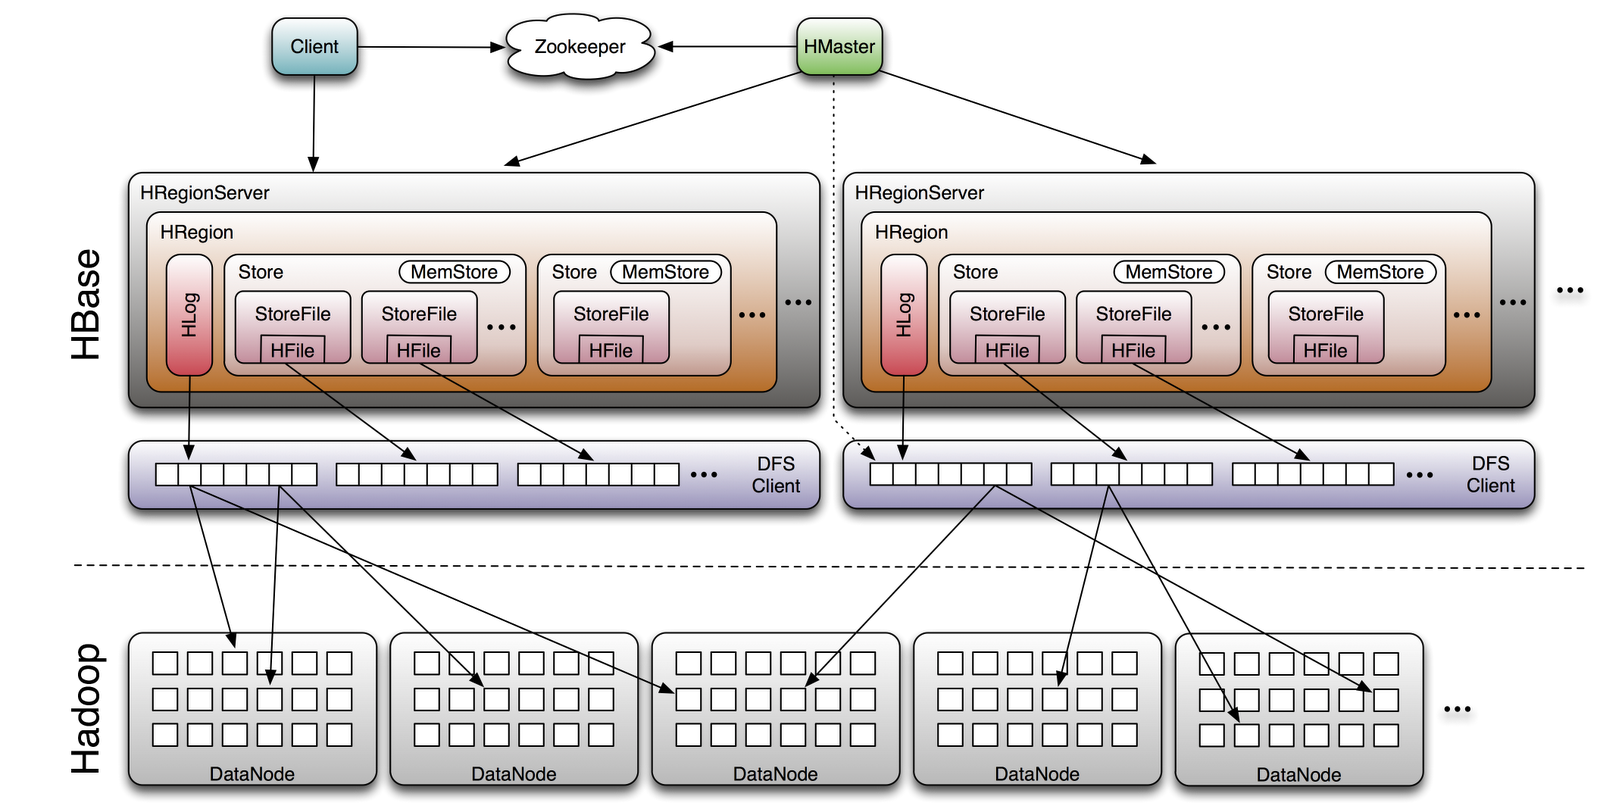
\includegraphics[height=6cm]{hbase-files}
}
\frame[t]{\frametitle{Running the Diagnostics}
      \begin{itemize}
        \item At Explorys we realized that the problems with running MapReduce over HBase stem from a common root.
        \item The batch processing data access pattern is conflated with a typical client read scenario. TableInputFormat is
          not some glorious miracle of backend data structures. It is actually very similar to how you might write it if it didn't exist.
        \item Each map task uses the client API to scan over the Results in the HBase table. The primary advantage over typical use is
          merely concurrent scans allowing parallelism. The overhead of the client server architecture is offset by a large amount of
          buffering to reduce the impact of Remote Procedure calls, but it is far from the mark of a direct file-system access even if the data is
          local to the MapReduce task.
      \end{itemize}
}


\section{Design}
\frame[t]{\frametitle{Direct Access}
  \begin{itemize}
    \item We wanted to design an InputFormat that allowed direct, read-only subscription to the StoreFiles for an HBase Table.
    \item Through some conversation with the HBase committers, especially St. Ack, we were told
      \begin{enumerate}
        \item We were crazy for thinking of this.
        \item More direct data access is something that's been requested before.
        \item We might have a viable approach by spinning up our own Region objects and using those to gain access to the underlying HFiles.
      \end{enumerate}
    \item There are a few contraindications to the approach that we will discuss later.
  \end{itemize}
}

\frame[t]{\frametitle{How to make this fast}
  \begin{itemize}
    \item Each storeFile is a column-family specific sorted list of KeyValues. The storefiles themselves are ordered by the timestamps.
    \item The approach is to treat each HFile as a heap of KeyValues. We then built an outerheap of HFiles where the comparator is
      the KeyValue.COMPARATOR applied to the top of the heap.
    \item Then we merge the results into a Result object as they are read in to provide the familiar pair of rowkey and Result object.
    \item Due to reverse timestamp sorting, Delete KeyValues (tombstone markers) will be encountered before the older records that they
      nullify.
  \end{itemize}
}

\frame[t]{\frametitle{Anatomy of an HFile \cite{SCHUBERT09,HBASEIO11}}
  \begin{columns}[t]
  \begin{column}{5cm}
  \begin{tabular}{|l|l|}
    \hline
    \multicolumn{2}{|c|}{A Typical HFile} \\
    \hline
   1 & Data Block 0 \\
    \hline
   2 &  Data Block 1 \\
    \hline
   3 & Meta Block \\
    \hline
   4 & File Info \\
    \hline
   5 & Data Block Index \\
    \hline
   6 & Meta Block Index \\
    \hline
   7 & Trailer \\
    \hline
  \end{tabular}
  \end{column}
  \begin{column}{5cm}
  \begin{tabular}{|l|l|}
    \hline
    \multicolumn{2}{|c|}{A Typical DataBlock} \\
    \hline
   1 & Data Block Magic \\
    \hline
   2 & Key Length \\
    \hline
   3 & Value Length \\
    \hline
   4 & Key \\
    \hline
   5 & Value \\
    \hline
   6 & Key Length \\
    \hline
   7 & Value Length \\
    \hline
   8 & Key \\
    \hline
   9 & Value \\
    \hline
   10 & ... \\
    \hline
   \end{tabular}
  \end{column}
  \end{columns}
}

\section{Running MapReduce directly over HFiles}
\frame[t]{\frametitle{Implementation}
  \begin{itemize}
    \item Here at Explorys, we implemented this proposed InputFormat to be used as a plug and play replacement for TableInputFormat.
    \item Almost...
    \item The code is hosted on github at \href{https://github.com/ExplorysMedical/Apothecary}{https://github.com/ExplorysMedical/Apothecary}
    \item Problems? Compaction and Region Splitting. Memstore access. Why?
  \end{itemize}
}

\frame[t]{\frametitle{Dealing with HBase Data Administration}

 \begin{enumerate}
    \item Turn off data source or funnel into temporary storage.
    \item Trigger flush and compaction.
    \item Wait for flush and compaction to finish. All the data is on disk.
    \item Create a log of the existing storefiles.
    \item Run the MapReduce Job
    \item Check the log to see that the state of the table didn't change (region splits or compaction).
    \item Possible do-over.
  \end{enumerate}
  \vspace{0.2cm}
 \begin{itemize}
  \item That's a lot. What can we skip?
  \item Hard links?
  \end{itemize}
}
\frame[t]{\frametitle{Performance}
   \begin{tabular}{|l|l|l|}
     \hline
      & TableInputFormat & HFiles \\
     \hline
     Copying a Table & 5:06 & 0:26 \\
     \hline
     Explorys Indexing Job & 1:50 & 0:30 \\
     \hline
   \end{tabular}
   \vspace{2cm}
   \begin{itemize}
     \item Better over large tables where cache doesn't have an impact.
     \item Worth the operation overhead in some circumstances.
     \item Major motivation for hard links and/or table snapshotting.
   \end{itemize} 
   {\tiny
   \begin{itemize}
     \item Indexing Job run with 800 input splits ~300 mappers.
     \item Copy Job run with 800 input splits, 95 concurrent Mappers.
   \end{itemize} 
   }
 }
\frame[t]{\frametitle{Problems}
  \vspace{0.5cm}
  \begin{itemize}
    \item Serious memory usage. HFile block indexes can be quite large, although needn't be loaded in full since HBase 0.92 \cite{HFILEV2}
    \item Operational constraints unwieldy. HBase Administration is asynchronous, doesn't return monitoring object.
    \item Tenuous relationship with non-exposed API. No guarantees that upgrades won't break it.
    \item Aside from compaction rearranging files, Memstore is not included. 
      We could possibly read WAL and construct our own memstore if compaction problem is solved..
  \end{itemize}
}
\frame[t,allowframebreaks]{\frametitle{References}
\bibliographystyle{amsalpha}
\begin{thebibliography}{1}
	{\small
          \bibitem{SCHUBERT09}
            Schubert Zhang (2009). HFile: A Block-Indexed File Format for Store Sorted Key-Value Pairs
            \href{http://www.slideshare.net/schubertzhang/hfile-a-blockindexed-file-format-to-store-sorted-keyvalue-pairs}{http://www.slideshare.net/schubertzhang/hfile-a-blockindexed-file-format-to-store-sorted-keyvalue-pairs}
          \bibitem{HBASEIO11}
            Matteo Bertozzi (2011). HBase I/O: HFile
            \href{http://th30z.blogspot.com/2011/02/hbase-io-hfile.html?spref=tw}{http://th30z.blogspot.com/2011/02/hbase-io-hfile.html?spref=tw}
          \bibitem{HFILEV2}
            Apache Software Foundation (2012). HBase Book: Appendix E. HFile format version 2
            \href{http://hbase.apache.org/book/hfilev2.html}{http://hbase.apache.org/book/hfilev2.html}
          \bibitem{LINELAND}
            Lars George (2009). HBase Architecture 101 -Storage
            \href{http://www.larsgeorge.com/2009/10/hbase-architecture-101-storage.html}{http://www.larsgeorge.com/2009/10/hbase-architecture-101-storage.html}
	}
\end{thebibliography}
}
\end{document}
